\section{Introduction}

3D visual grounding maps a referring expression to one object in a reconstructed 3D scene. A system that receives ``the chair next to the desk'' must recognize candidate chairs, identify plausible desk anchors, and reason about the spatial relation between them. The task is therefore more structured than ordinary object classification: many examples are only resolvable through relation evidence, same-class distractor handling, and a speaker-dependent interpretation of spatial language.

This project studies that relational part of 3D grounding. The initial goal was to build a relation-aware grounding model that improves over a reproduced ReferIt3DNet-style listener. The repository has since evolved into a broader empirical study with scene-disjoint split recovery, frozen-logit baseline evaluation, hard-subset diagnostics, coverage analysis, dense reranking experiments, viewpoint-conditioned ablations, counterfactual training pilots, and latent relation-mode pilots. This report follows the current evidence rather than the original hypothesis: the best-supported contribution is \method{}, not explicit viewpoint supervision or completed anchor-chain reasoning.

This project contributes three course-level artifacts: a verified scene-disjoint evaluation pipeline, a diagnostic suite for hard-subset and anchor-coverage failures, and a controlled conditioned relation-scoring study. It is therefore framed as a reproducible empirical study with a conservative method signal, rather than as a state-of-the-art 3D grounding system.

\begin{figure}[!htbp]
  \centering
  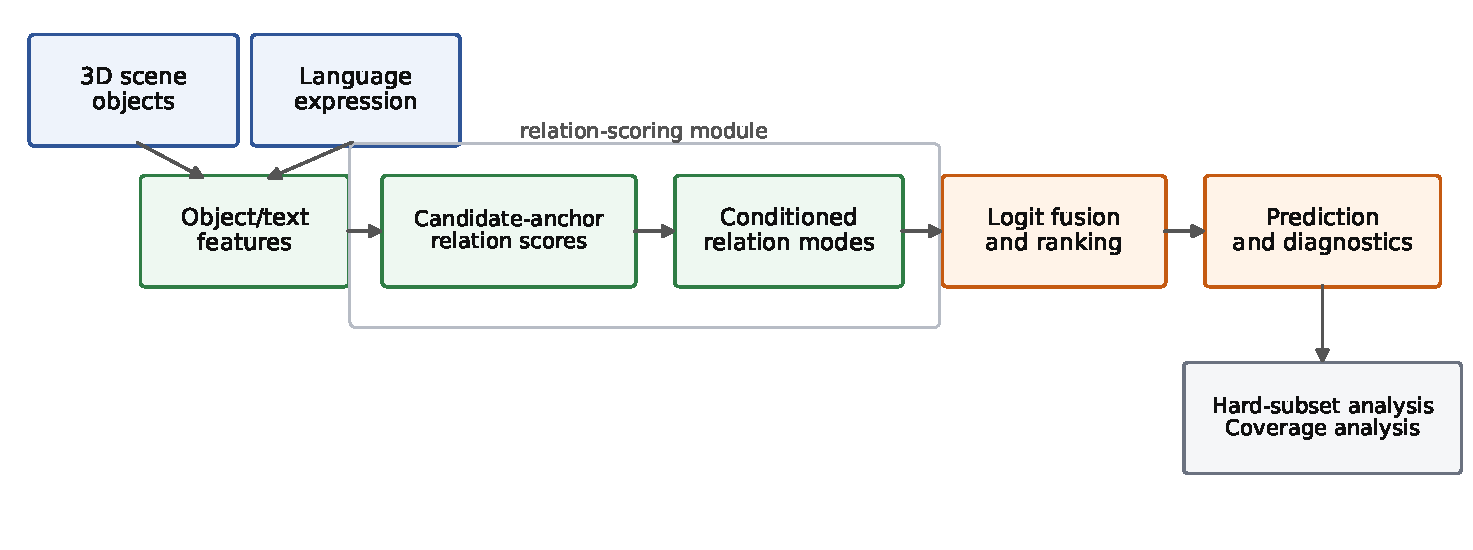
\includegraphics[width=\linewidth]{../../assets/figures/figure1_pipeline.pdf}
  \caption{Current project pipeline. The system keeps the object-centric grounding setup, adds relation-aware scoring over candidate-anchor pairs, and reports both predictions and diagnostics. The strongest method evidence supports a conditioned relation architecture, while the broader project contribution includes scene-disjoint evaluation and failure analysis.}
  \label{fig:pipeline}
\end{figure}

The project has three current-evidence conclusions. First, scene-disjoint grounding failures are concentrated in measurable hard subsets, especially same-class clutter and multi-anchor references. Second, sparse geometric anchor selection creates a real coverage bottleneck: dense all-pair candidate-anchor scoring can include anchor evidence that sparse top-$k$ selection misses. Third, the controlled method evidence supports conditional relation computation, but it does not support the claim that explicit viewpoint supervision is the source of the gain.

This distinction matters for a research-oriented course project. A less careful report could claim that viewpoint labels solve relational grounding. The current results do not justify that. Instead, the repository shows a more realistic research process: reproduce a baseline, identify where it fails, test relation mechanisms, preserve negative findings, and reframe the method claim when ablations contradict the initial explanation.

\paragraph{Code availability.}
Code and reproducibility artifacts are available at:\\
\url{https://github.com/checheng117/relation-aware-3d-grounding}.
